\documentclass{article}


% if you need to pass options to natbib, use, e.g.:
%     \PassOptionsToPackage{numbers, compress}{natbib}
% before loading neurips_2023


% ready for submission
\usepackage[final, nonatbib]{neurips_2023}


% to compile a preprint version, e.g., for submission to arXiv, add add the
% [preprint] option:
%     \usepackage[preprint]{neurips_2023}


% to compile a camera-ready version, add the [final] option, e.g.:
%     \usepackage[final]{neurips_2023}


% to avoid loading the natbib package, add option nonatbib:
%    \usepackage[nonatbib]{neurips_2023}


\usepackage[utf8]{inputenc} % allow utf-8 input
\usepackage[T1]{fontenc}    % use 8-bit T1 fonts
\usepackage{hyperref}       % hyperlinks
\usepackage{url}            % simple URL typesetting
\usepackage{booktabs}       % professional-quality tables
\usepackage{amsfonts}       % blackboard math symbols
\usepackage{nicefrac}       % compact symbols for 1/2, etc.
\usepackage{microtype}      % microtypography
\usepackage{xcolor}         % colors

\usepackage[spanish, es-tabla]{babel}

\usepackage[pdftex]{graphicx}
\usepackage{pgf}
\usepackage{subcaption}
\graphicspath{{./graphs/}}

%% biblatex
\usepackage[style = numeric, backend = biber, sorting = none, doi = false, isbn = false, url = true]{biblatex}
% \usepackage[defernumbers = true, style = numeric, backend = biber, sorting = none, doi = false, isbn = false, url = true]{biblatex}
% \usepackage[style = numeric, backend = biber, sorting = none]{biblatex}    % REFERENCIAS como section
\AtEveryBibitem{
    \clearfield{urlyear}
    \clearfield{urlmonth}
} % Do not show the "(visited on <date>)" on the references
\DefineBibliographyStrings{spanish}{}
\usepackage{csquotes}
\addbibresource{./dmcyt.bib}
\renewcommand*{\bibfont}{\fontsize{9}{12}\selectfont}



\title{Grafos en neurociencias (pre TP2)}

\author{
  Víctor A.~Bettachini\\ %\thanks{Use footnote for providing further information about author (webpage, alternative address)---\emph{not} for acknowledging funding agencies.} \\
  Datamining en ciencia y tecnología 2023\\
  Especialización en Explotación de Datos y Descubrimiento del Conocimiento\\
  \texttt{bettachini@gmail.com}
}


\begin{document}


\maketitle


% \begin{abstract}
%?
%\end{abstract}


% Enunciado
% Se sugiere realizar la entrega en formato latex, pero en este caso va a ser optativo (en el TP ya es obligatorio, sugerimos que lo usen de práctica). Pueden acceder a formatos de distintas conferencias a través de Overleaf, en particular les sugerimos el formato de NeurIPS que es una de las conferencias más importantes en IA.
% Se sugiere un máx de 4 carillas (mín 2), no se debe incluir código a menos que sea algo esencial que hayan desarrollado ustedes (es preferible en este caso incluir el pseudo-código). Aclaración: No vamos a corregir código en la entrega.
% El pre TP es individual.


% \section{Introducción}

\section{Materiales y métodos}

\paragraph{Datos}
Se hace uso de datos producto de la medición de la señal de resonancia magnética funcional (fMRI).
Definidos 116 volúmenes de interés del cerebro en términos de su activación \cite{tzourio-mazoyer_automated_2002}, se publicaron coeficientes de correlación lineal entre sus medias en distintos segmentos temporales \cite{tagliazucchi_large-scale_2013}.
Con estos datos se generó una matriz de correlación, y a partir de la misma los grafos analizados en este trabajo.


\paragraph{Recurso informático} 
Un cuaderno (notebook) Jupyter provisto por los docentes en el sitio web denominado ``Campus'' \cite{kamienkowski_curso_2023} es la plantilla donde se escribió código en lenguaje Python.
Este explotó funciones de las biblioteca NetworkX \cite{hagberg_exploring_2008}.



\subsection{Preprocesamiento de los datos}
% Cada actividad realizada se describe bajo los titulos que figuran en el enunciado del trabajo práctico publicado en el

\paragraph{Carga del conjunto de datos} 
Los archivos provistos corresponden a los estadios de sueño N1, N2, N3 y despierto (W) para 18 sujetos.
Estos estuvieron acompañados de una tabla que describe la denominación y  ubicación espacial las regiones en que se parcializó el cerebro.



\section{Resultados}

\subsection{Manipulación de datos}

\paragraph{Matriz de correlación}
La matriz de adyacencia pesada que muestra la figura \ref{fg:matriz_correlación_pesada} corresponde a la condición de despierto para el sujeto número 2.

Una medida que caracteriza un grafo es la densidad, $\delta$, definida como la razón entre los enlaces presentes sobre todos los posibles en el grafo.
Para convertir la matriz en una de adyacencia binaria con una densidad de enlaces \(\delta = 0.8\) se discriminaron sus pesos con un umbral \(0.77997\) y así se obtuvo la matriz que muestra la figura \ref{fg:matriz_correlación_binaria}.

\begin{figure}[ht]
	\centering
	\begin{subfigure}[b]{0.3\textwidth}
		\includegraphics[width= \linewidth]{matriz_correlación}
		\caption{Pesada}
		\label{fg:matriz_correlación_pesada}
	\end{subfigure}
	\begin{subfigure}[b]{0.25\textwidth}
		\includegraphics[width= \linewidth]{matriz_correlación_binaria}
		\caption{Binaria}
		\label{fg:matriz_correlación_binaria}
	\end{subfigure}
	\caption{Matrices de correlación de las medias de señales para el sujeto número 2 despierto. 
	}
	\label{fg:matriz_correlación}
\end{figure}


\paragraph{Grafo de la matriz de adyacencia binaria}
No es totalmente conectado.
Hay tres componentes conectadas de 92, 5 y 2 nodos en tanto que los 17 restantes están aislados.
La distancia mínima entre nodos contabiliza cuantos intermedios deben atravesarse para ir de un nodo a otro.
Esta medida para los aislados no tiene sentido, por lo en este grafo no puede obtenerse una distancia media $d$ a lo fines de tener una media de que tan ``conectado'' se presenta el grafo.
Una medida alternativa es la eficiencia global.
% Para el conjunto, no conectado, este valor parece bajo, $\approx 8\%$.
% Y en el componente mayoritario, el de 92 nodos, este valor apenas se incrementa hasta un $\approx 12\%$. 


\paragraph{Eficiencia global de conectividad}
La suma de la inversa de es una medida de la eficiencia de conectividad global del grafo, $\mathrm{eff} = \frac{1}{n (n-1)} \sum_{i \neq j} \frac{1}{d(i,j)}$ \cite{ek_global_2015}.
%Puesto que la razón de normalizar por $n (n-1)$ es para que la eficiencia de un grafo totalmente conectado sea $1$, en este grafo que no es totalmente conectado, realicé una estimación forma manual sobre la suma se realiza sobre los nodos que efectivamente están conectados.
% Sumando la inversa de las distancias de los enlaces presentes y normalizando por su número se obtuvo un valor de $\mathrm{eff} \approx 0.389$.
% No logré realizar un cálculo manual en línea con valores publicados para esta medida, pero 
La biblioteca NetworkX provee una función que la calculó en $\approx 0.245$.


\paragraph{Distribución de grado}
El número de enlaces por nodo, o grado $k$, se distribuye en forma dispar.
De un total de $534$ enlaces el grado mayor resultó $k_\textnormal{máx} = 30$, y un relativamente alto promedio $\langle k \rangle \approx 9.207$ aunque no hay que olvidar que no participan aquí los nodos aislados.
El histograma de $k$ que muestra la figura \ref{fg:hist_k} que este $\langle k \rangle$ es representativo de la distribución.

En una medida similar a la densidad que cuenta la proporción de enlaces sobre los posibles puede hacerse algo similar calculando la proporción de cuantos de los posibles enlaces entre primeros vecinos efectivamente se realizan.
Esto se denomina coeficiente de agrupamiento (\emph{clustering}) por nodo $C_i$, cuyo promedio para este grafo es $\langle C_i \rangle \approx 0.527$. 
Coloreando cada nodo según su $C_i$ y ubicándole por las coordenadas (y,z) en el cerebro se obtiene la figura \ref{fg:clustering}. 

\begin{figure}[ht]
	\centering
	\begin{subfigure}[b]{0.25\textwidth}
		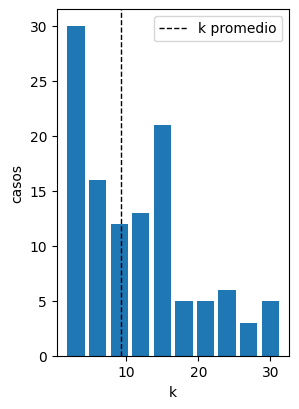
\includegraphics[width= \linewidth]{histograma_k}
		\caption{Histograma para $k$.
		}
		\label{fg:hist_k}
	\end{subfigure}
	\begin{subfigure}[b]{0.7\textwidth}
		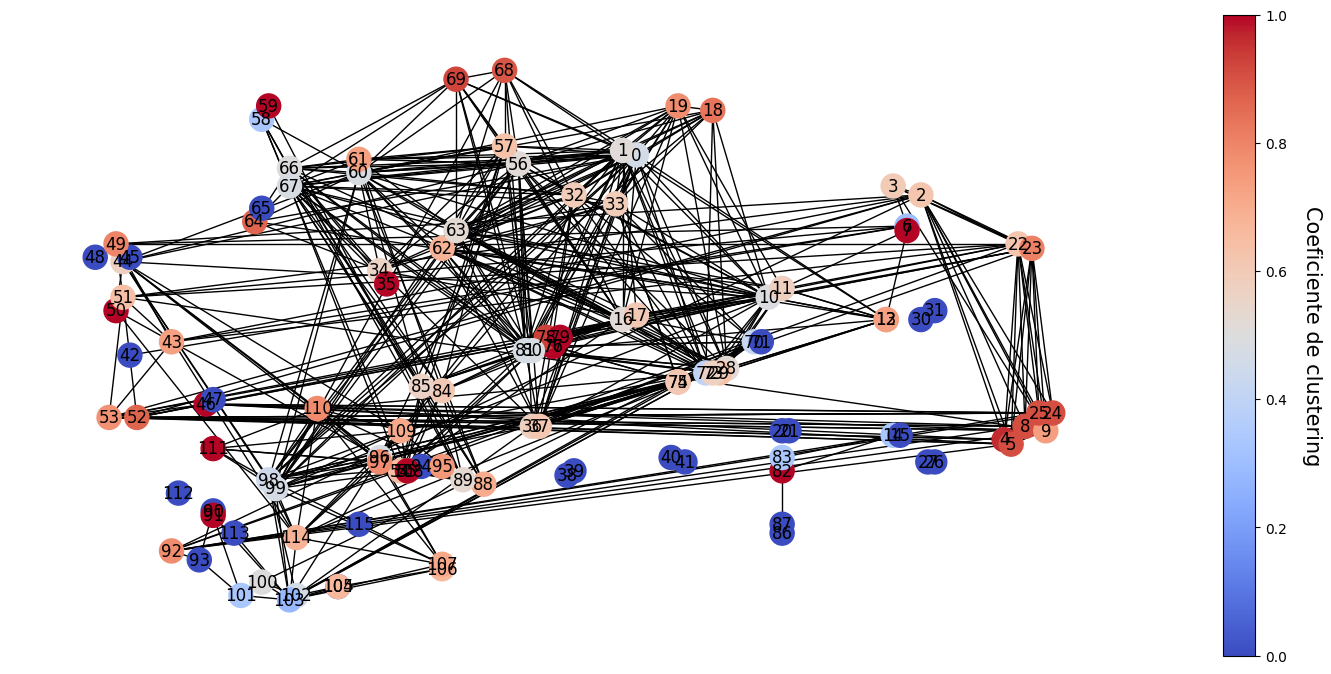
\includegraphics[width= \linewidth]{clustering}
		\caption{número de nodo $i$ y su $C_i$.
		}
		\label{fg:clustering}
	\end{subfigure}
	\caption{Distribución de grado y coeficiente de agrupamiento.
	}
	\label{fg:distribución_de_grado}
\end{figure}


\paragraph{Grafos prototípicos}
Tres algoritmos generaron grafos de conexiones entre el mismo número de nodos, $n = 116$, que de la matriz de adyacencia binaria.
Se buscó que estos presente coeficientes de caracterización similares al del grafo de esta.

El \textbf{algoritmo de Erdös–Rényi} enlaza un par de nodos si una probabilidad al azar supera un umbral \cite[sección 3.2]{albert-laszlo_barabasi_network_2016}.
Estableciendo en función del $\langle k \rangle$ de la red original tal probabilidad como $p = \frac{\langle k \rangle}{n -1}$ se obtuvo una densidad prácticamente idéntica $\delta = 0.0808$ a la de la red original, $0.0801$, con una suma de enlaces, $539$, también muy cercana, $534$. 
El coeficiente de agrupamiento $\langle C_i \rangle = 0.7986$ resulta bastante disímil con el $0.5271$ de la red original.
Esta red azarosa, a diferencia de la original, mostró estar totalmente conectada, como se aprecia en la figura \ref{fg:erdos_renyi}. 
En contrapartida, las redes reales suelen estar particionadas en múltiples componentes conectadas \cite[sección 3.7]{albert-laszlo_barabasi_network_2016}.

Si una red fuera perfectamente regular y todos los nodos tuvieran idéntica $k$, la distancia mínima entre dos nodos $d$, es decir cuantos intermedios debe atravesarse para enlazar uno con otro, seguiría una dependencia polinomial con $n$.
En las redes reales $d$ presenta una dependencia mucho menor con $n$, con $\log(n)$ de hecho.
Este fenómeno recibe el nombre de \emph{mundo pequeño}, o \emph{small-world}, por la sorpresiva poca distancia entre dos cualesquiera nodos de la red.
Asimismo, en las reales, el coeficiente de agrupamiento $C_i$ suele ser más alto que en una red azarosa \cite[sección 3.9]{albert-laszlo_barabasi_network_2016}. 
En respuesta a estas observaciones, el \textbf{algoritmo de Watts-Strogatz} extiende el modelo de un $k$ regular con una probabilidad de que un enlace cambie a nodo, lo que genera redes intermedias entre una regular y una azarosa.
El número de enlaces total más cercano al de la red original, $580$, se obtuvo con $k = \mathrm{entero}(\langle k \rangle) + 1$. 
Puesto que la $\delta = 0.870$ es insensible al parámetro de reconexión se lo ajustó buscando un $\langle C_i \rangle$ similar al de la red original.
Este fluctúa por efectos azarosos pero se logró que este oscilara en torno al $\approx 0.527$ con una probabilidad de reconexión de $0.815$.
Pero la red generada se presenta totalmente conectada y con un aspecto muy diferente a la original, como muestra la figura \ref{fg:watts_strogatz}. 
Se pude generar una red con aspecto más similar incrementando la reconexión y así haciéndola más azarosa y similar a la de las mediciones, pero el resultante $\langle C_i \rangle$ se aleja del de esta.

Hasta aquí había esquivado el tratar la distribución de los grados $k$ según el modelo prototípico de red.
El proceso proceso binomial de una red azarosa para un $n \gg <k>$ presenta una distribución de Poisson \cite[sección 3.4]{albert-laszlo_barabasi_network_2016}.
Se comentó ya el fenómeno de \emph{mundo pequeño}, pero no el los menores $d$ son fruto de la existencia de nodos con alto $k$ llamados \emph{hubs}.
La distribución de probabilidad de $k$ se extiende mostrando frecuentemente una dependencia con una ley de potencias $p_k \sim k^{- \gamma}$, dando origen al designación de redes \emph{sin escala} o \emph{scale-free} \cite*[sección 4.2]{albert-laszlo_barabasi_network_2016}.
El \textbf{algoritmo de Barabási-Albert} genera tales redes a partir de un parámetro $m$ que determina cuantos enlaces se agregan en cada paso.
Se ajustó $m = \mathrm{entero} \left( \frac{\langle k \rangle}{2} \right) + 1$ para dar cuenta de no contar dos veces el número medio de enlaces de la red original y el uno adicional se agregó para que la red resultante tuviera el número de enlaces más similar a esta ($555$).
Lo generado presentado en la figura \ref{fg:barabási_albert} también muestra una red conectada, pero con una similitud adicional con la original al mostrar claros \emph{hubs}.  

\begin{figure}[ht]
	\centering
	\begin{subfigure}[b]{0.32\textwidth}
		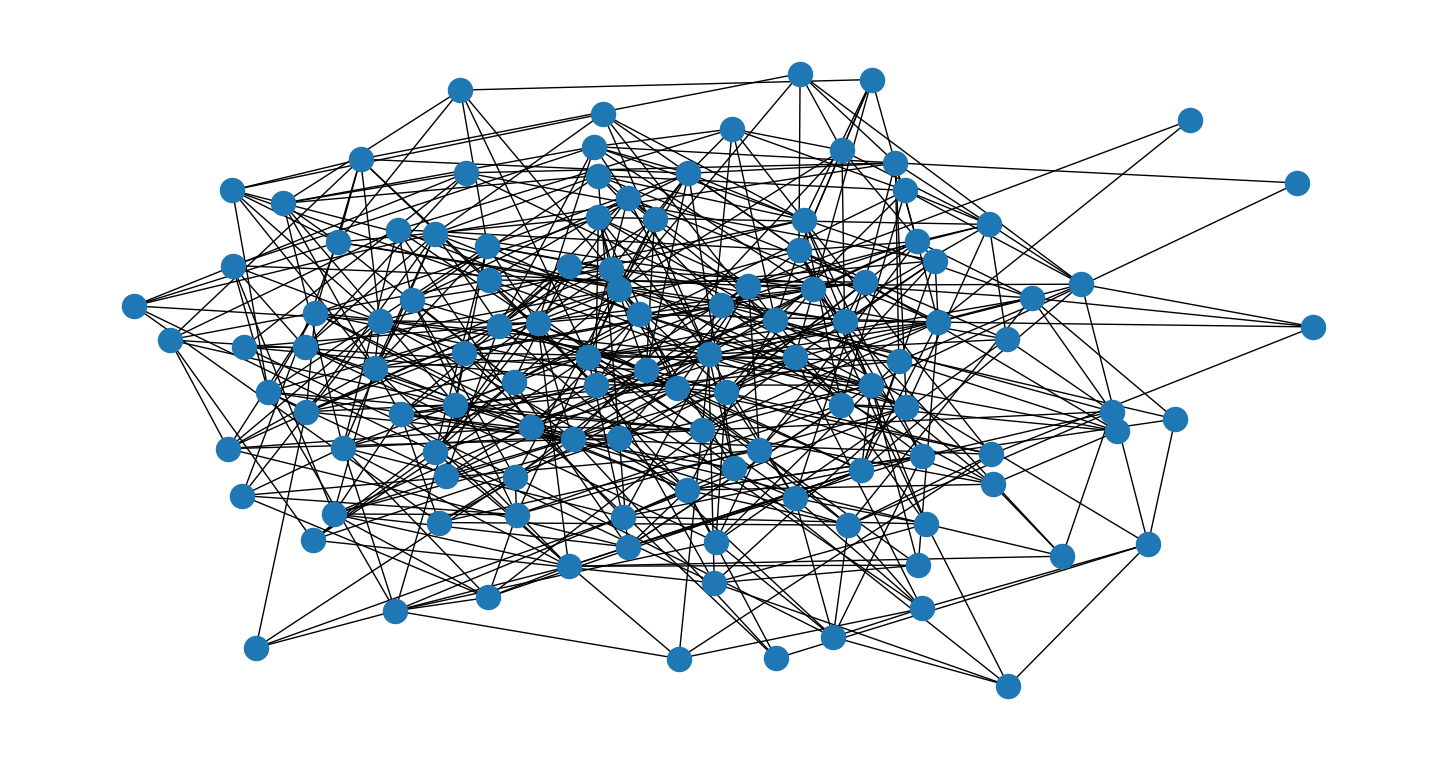
\includegraphics[width= \linewidth]{erdos_renyi}
		\caption{Azarosa}
		\label{fg:erdos_renyi}
	\end{subfigure}
	\begin{subfigure}[b]{0.32\textwidth}
		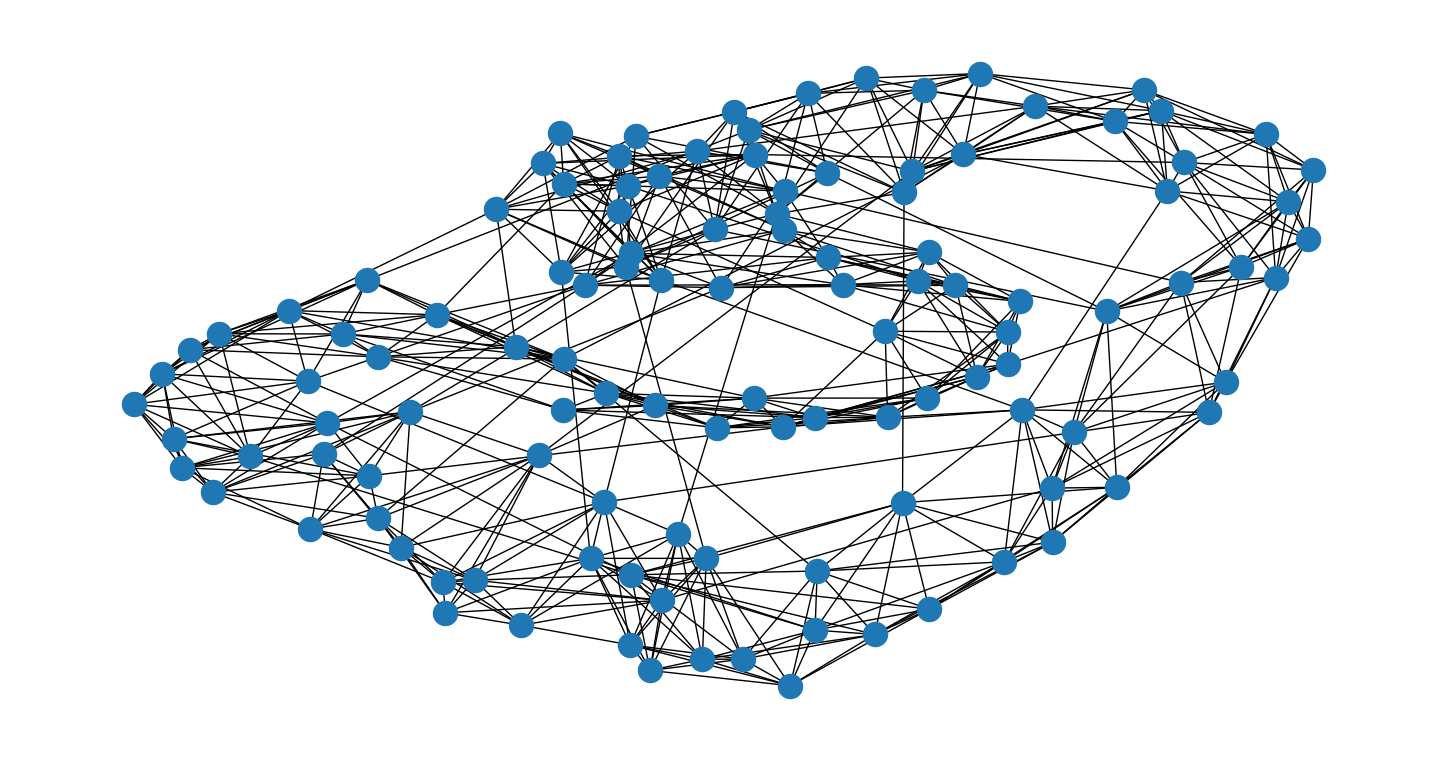
\includegraphics[width= \linewidth]{watts_strogatz}
		\caption{Mundo pequeño}
		\label{fg:watts_strogatz}
	\end{subfigure}
	\begin{subfigure}[b]{0.32\textwidth}
		\includegraphics[width= \linewidth]{barabási_albert}
		\caption{Sin escala}
		\label{fg:barabási_albert}
	\end{subfigure}
	\caption{Grafos generados respetado el número de nodos y aproximadamente el de enlaces de la red original con algoritmos de (a) Erdös–Rényi, (b) Watts-Strogatz y (c) Barabási-Albert.}
	\label{fg:prototípicas}
\end{figure}



\paragraph{Coeficientes de grafos prototípicos}

Las redes prototípicas comentadas en la sección anterior son una realización al azar.
Para dar respuesta a que tan similares son los coeficientes que les caracterizan a los de la red producto de las mediciones se hicieron 1000 corridas de estos algoritmos a lo fines de realizar histogramas de del número medio de enlaces, $<k>$, el máximo número de estos, $\textnormal{máx} k$, el coeficiente de agrupamiento medio, $\langle C_i \rangle$, y la eficiencia de conectividad, $\mathrm{eff}$.

En el caso de las redes azarosas generadas con el algoritmo de Erdös–Rényi, la figura \ref{fg:hist_poisson} muestra que el $<k>$ y los $\textnormal{máx} k$ los exceden ligeramente.
Pero los $\langle C_i \rangle$ están muy por debajo y la $\mathrm{eff}$ por arriba de los de la red original indicados con líneas punteadas verticales.
Lo primero no es extraño pues de hecho las redes al azar presentan sistemáticamente un $\langle C_i \rangle$ menor que las reales \cite[sección 3.9]{albert-laszlo_barabasi_network_2016}.
Para Lo segundo espera un resultado opuesto, pues en las redes reales $d$ son menores que en la red azarosa esperaba que la suma de sus inversas fuera menor que en la red producto de las mediciones.
Pienso que estoy cometiendo un error aquí.

\begin{figure}[ht]
  \centering
  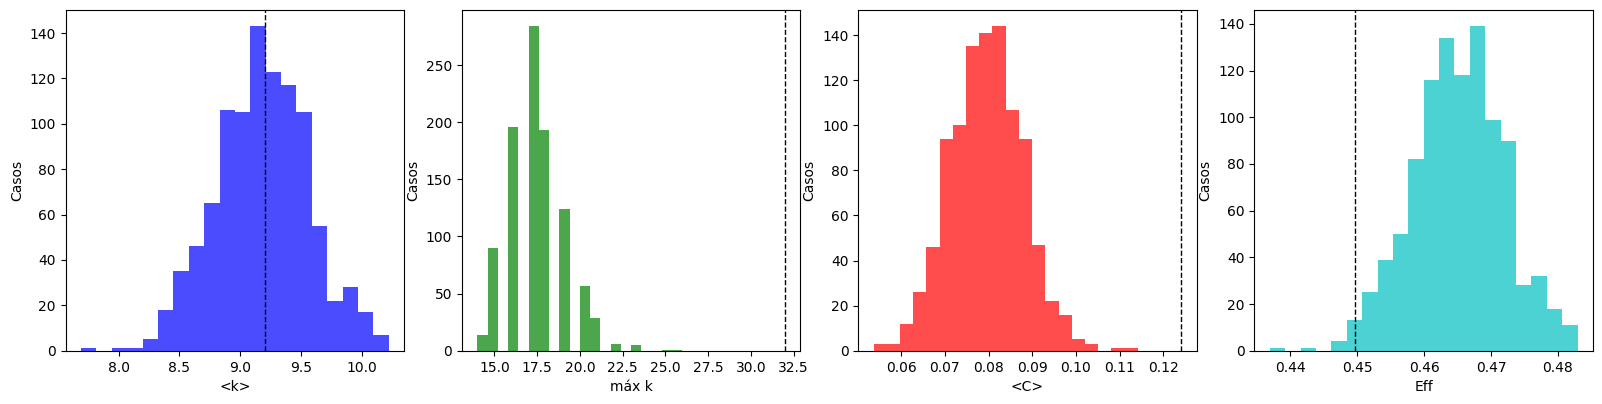
\includegraphics[width= \linewidth]{hist_poisson}
  \caption{Magnitudes de las redes azarosas.}
	\label{fg:hist_poisson}
\end{figure}

En el caso de las redes generadas con el algoritmo de Watts-Strogatz, la figura \ref{fg:hist_small_world} muestran un $\langle k \rangle$ superior al de la red producto de las mediciones pero unos $\textnormal{máx} k$ comparables.
Puesto que se ajustó para que así fuera la concordancia con el coeficiente de agrupamiento medio es buena.
Nuevamente la eficiencia global arroja un valor mucho mayor que el de la red original que no puedo explicar.
Si no fuera por este desarreglo la red del tipo \emph{mundo pequeño} sería una buena candidata para representar el fenómeno que dio origen a la red original.

\begin{figure}[ht]
  \centering
  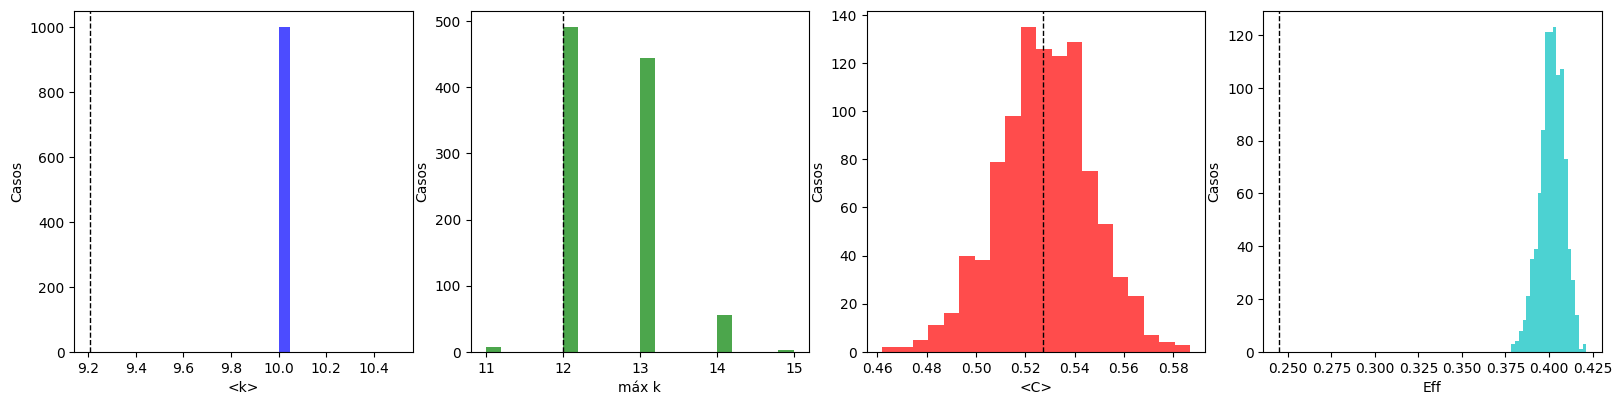
\includegraphics[width= \linewidth]{hist_small_world}
  \caption{Magnitudes de las redes \emph{mundo pequeño}.}
	\label{fg:hist_small_world}
\end{figure}

En el caso de las redes generadas con el algoritmo de Barabási-Albert, la figura \ref{fg:hist_scale_free} muestran un $\langle k \rangle$ superior al de la red producto de las mediciones y unos $\textnormal{máx} k$ un tanto mayores pero comparables.
En contrapartida el coeficiente de agrupamiento medio es mucho menor que el de la red original.
Y nuevamente no puedo explicar la eficiencia global mayor que la de la red original.

\begin{figure}[ht]
  \centering
  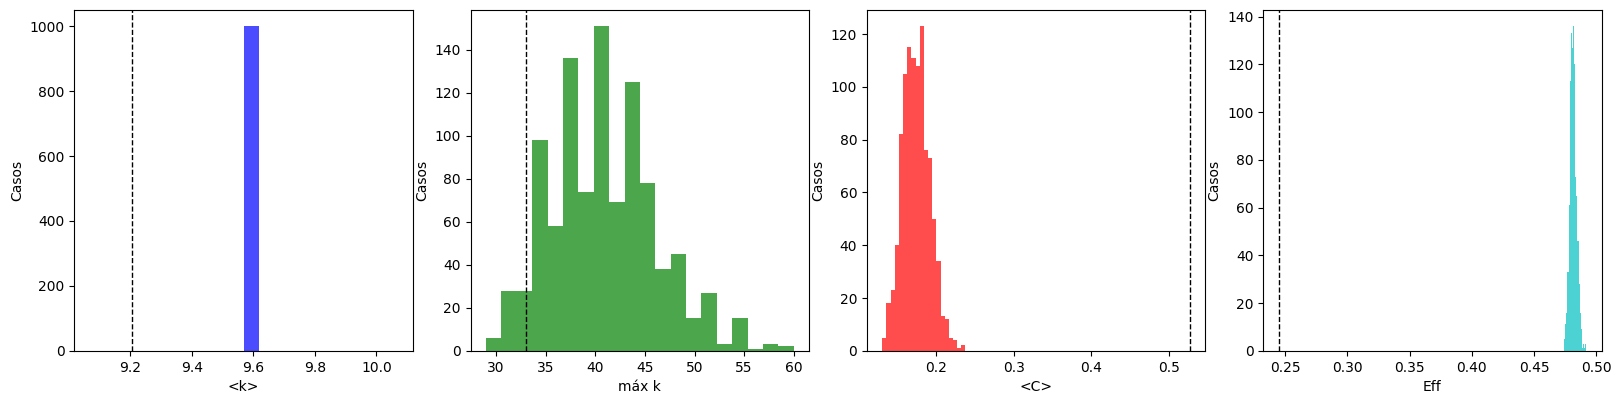
\includegraphics[width= \linewidth]{hist_scale_free}
  \caption{Magnitudes de las redes \emph{sin escala}.}
	\label{fg:hist_scale_free}
\end{figure}




% \section{Discusión y conclusiones}

\printbibliography[title= Referencias, heading=bibintoc]

\end{document}
